%Tasks under GBYP Modelling for 2013, identified at Gloucester Meeting


\subsection{Objectives}

In 2013 the SCRS elaborated a work plan for 2014 which included a data preparatory meeting to incorporate the new catch and effort information in ICCAT databases and continuing working on new modeling platforms and inputs in a view to minimize uncertainties in the 2015 and ongoing assessments. The work plan approved by the SCRS did not include an update of the stock assessment in 2014, as stated by the ICCAT Recommendation [12-03] for the eastern Atlantic and Mediterranean bluefin tuna. This decision was based in the lack of SCRS resources for conducting the update and undertaking the difficult task of preparing the 2015 assessment. 

Nevertheless, the Commission at its 23th Regular Meeting requested the SCRS to implement Rec. [12-03], i.e., to update the stock assessment of East Atlantic and Mediterannean bluefin tuna. The following year the Commission also adopted Recommendation 13-09 which states: “In 2014, the SCRS will update the stock assessment for bluefin tuna for the western Atlantic stock”.

Hence, the work plan developed by the Bluefin tuna species group for 2014 has needed to be modified to include in 2014 an update of both the West and the East Atlantic and Mediterranean stock assessments and the corresponding data preparatory work. The new work plan elaborated by the Bluefin rapporteurs and the SCRS Chair is attached as Annex 1. 

Following the revised work plan the objectives of this data preparatory meeting are the following: 

\begin{enumerate}[1.]
\item Update fishery indicators in accordance Rec. [12-03], paragraph. 50. 
\item Revise Task II by validating and integrating the catch at size statistics with new information from farms and other sources of information. 
\item Update the length-weight relationship for both stocks, i.e. Western and Eastern / Mediterranean stocks. 
\item Define the procedure to prepare CAS, CAA, WAA (total and per fleet) using the new length-weight relationship. 
\item Review tagging past and recent data for bluefin tuna.
\item Complete outstanding tasks from the Biological Parameters meeting in Tenerife (age-length relationships, morphometric conversions, natural mortality, reproduction, etc.). 
\end{enumerate}

\subsection{Tentative Agenda}

\begin{enumerate}[1.]
\item Opening, adoption of the Agenda and meeting arrangements.
\item Review of historical and new information on biology
\item Review of old and new Task I after the incorporation of new information from GBYP and other sources
\item Review of old and new Task II catch/effort data after the incorporation of new information from GBYP and other sources 
\item Review of old and new Task II size data 

\begin{enumerate}[5.1]
\item 5.1 Review of new information from farms and other sources
\item 5.2 Validation of the procedure followed to incorporate the information from farms and other sources into the ICCAT data base
\end{enumerate}

\item Definition of a new procedure to estimate CAS, CAA and WAA using new information validated by the Group
\item Review of available indices of relative abundance by fleet 
\item Definition of data inputs and specifications for the 2014 update assessment and advice framework.  
\item Identification of the evaluation team and definition of the revision procedure
\item  Develop a web app from the R-VPA2-BOX interface
\item Responses to the Commission
\begin{enumerate}[11.1]
\item Develop updated growth tables
\end{enumerate}
\item Recommendations
\item Other matters
\item Adoption of the report and closure
\end{enumerate}

\subsection{2014 Bluefin Tuna Work Plan}

Recommendation [10-04] states “In 2012, and thereafter every three years, the SCRS will conduct a stock assessment for bluefin tuna for the western Atlantic and eastern Atlantic and Mediterranean and provide advice to the Commission on the appropriate management measures, inter alia, on total allowable catch levels for those stocks for future years.” 

The Atlantic-wide Research Program for Bluefin tuna (GBYP) and various National programs have produced, and continue to produce, a great deal of new information on the biology and fisheries for bluefin tuna. In preparation for the planned 2015 assessment, time and resources of the SCRS are thus required to validate these data and to incorporate them in the ICCAT database as well as working on updated biological parameters and new modeling approaches. Therefore, the SCRS planned for several meetings in the 2012 work plan. The first two took place in 2013 and aimed at updating the biological parameters and comparing various modeling platforms. For 2014, the SCRS planned a data preparatory meeting (5-10 May) to incorporate the new catch and effort information in ICCAT databases and continuing working on new modeling platforms. 

Recommendation [12-03] for the eastern Atlantic and Mediterranean bluefin tuna further states “In 2014 the SCRS will conduct an update of the stock assessment and provide advice to the Commission.../... Furthermore, the SCRS shall work towards the development of new assessment modeling approaches and inputs, in a view to minimize uncertainties, which shall be used in a stock assessment in 2015 and thereafter every three years.” Finally, at its last session the Commission also adopted Recommendation 13-09 which states: “In 2014, the SCRS will update the stock assessment for bluefin tuna for the western Atlantic stock”.

To accommodate priorities to improve the scientific advice by 2015 and the latest commission requests, the SCRS proposes the following workplan for 2014, adapted from the plan approved by the SCRS in 2013:

\begin{enumerate}[1.]
\item Conduct an Inter-sessional Preparatory Workshop in early 2014 (6 days) that will focus on the following: 
\begin{enumerate}[a)]
\item Update fishery indicators in accordance Rec. [12-03], paragraph. 50, except for the Spanish bait boat CPUE as their quota has been transferred to Spanish purse seiners since 2012. The Japanese CPUE will have to be split into two periods, before and after TAC implementation due to changes in spatial coverage of the fishery. 
\item Revise Task II by validating and integrating the catch at size statistics with new information from farms and other sources of information. 
\item Update the length-weight relationship for both stocks, i.e. Western and Eastern / Mediterranean stocks. 
\item Prepare CAS, CAA, WAA (total and per fleet) using the new length-weight relationship. 
\item Review tagging past and recent data for bluefin tuna.
\item Complete outstanding tasks from the Biological Parameters meeting in Tenerife (age-length relationships, morphometric conversions, natural mortality, reproduction, etc.). 
\end{enumerate}
\item Continue a series of workshops and related activities (to be sponsored by the GBYP and various national programs) in accordance with recommendations from the Biological Parameters Meeting (Tenerife) and the Bluefin Methods meeting (Gloucester) including:
\begin{enumerate}[a)]
\item Establish a reference collection for otoliths and hard parts and calibrate age estimates among readers.
\item Larval biology workshop.
\item Continue the development of new modeling platforms that can better take into account various sources of uncertainties.
\end{enumerate}
\item Update the 2012 assessments of western and eastern/Mediterranean bluefin tuna using, insofar as is possible, the methods used during 2012.
\end{enumerate}


There is thus a considerable amount of work to be done in 2014, i.e., validating and incorporating 10,000s of new files into the current ICCAT databases, calibrating and updating all the size and age conversion methods, updating previous assessments and continuing the development of new modeling platforms.

The work plan for 2014 is detailed in a table of the main tasks, responsibilities, deadlines and priorities which is provided as an annex to this document. The first priority will be to conduct an update of the 2012 stock assessment for western and eastern/Mediterranean stocks using catch data and abundance indices updated through 2013. The second priority will be to incorporate the new information (trade, farms, biology) into the Task I and Task II data base (catch, catch-at-size, catch-at-age, weight-at-age). A preliminary assessment of the eastern/Mediterranean stock based on these revised Task I and Task 2 data will be attempted, but priority will be given to completing the update assessment stipulated by the relevant Commission Recommendations”. This line of priorities defines the order of the work that will be undertaken. Each priority must be completed in order for the group to move forward to the next step. The SCRS proposes that an additional inter-sessional meeting be planned in September 2014, during the species group meetings, to conduct the update of the 2012 stock assessment of eastern and western Atlantic stocks and, if time permits, a preliminary new assessment for the eastern stock. . This new preliminary stock assessment for the East will apply the current VPA software (VPA-2BOX) to the revised catch data using the new information (farm, trade, biological parameters). Initial ‘pilot’ updates of the 2012 SA (east and west) and the new preliminary SA for the East will be completed before the species group by the co-chairs and volunteer scientists and circulated prior to the species group meeting in September as an SCRS document. Any proposed revisions to the assessment will be addressed during the beginning of the Bluefin species group meeting to allow time for any additional runs and incorporation of the results into the executive summary. However, even if the new data are available this new stock assessment is unlikely to reduce substantially most of the unquantified uncertainties.

The following table summarized the activities defined in the work plan and its priorities. 


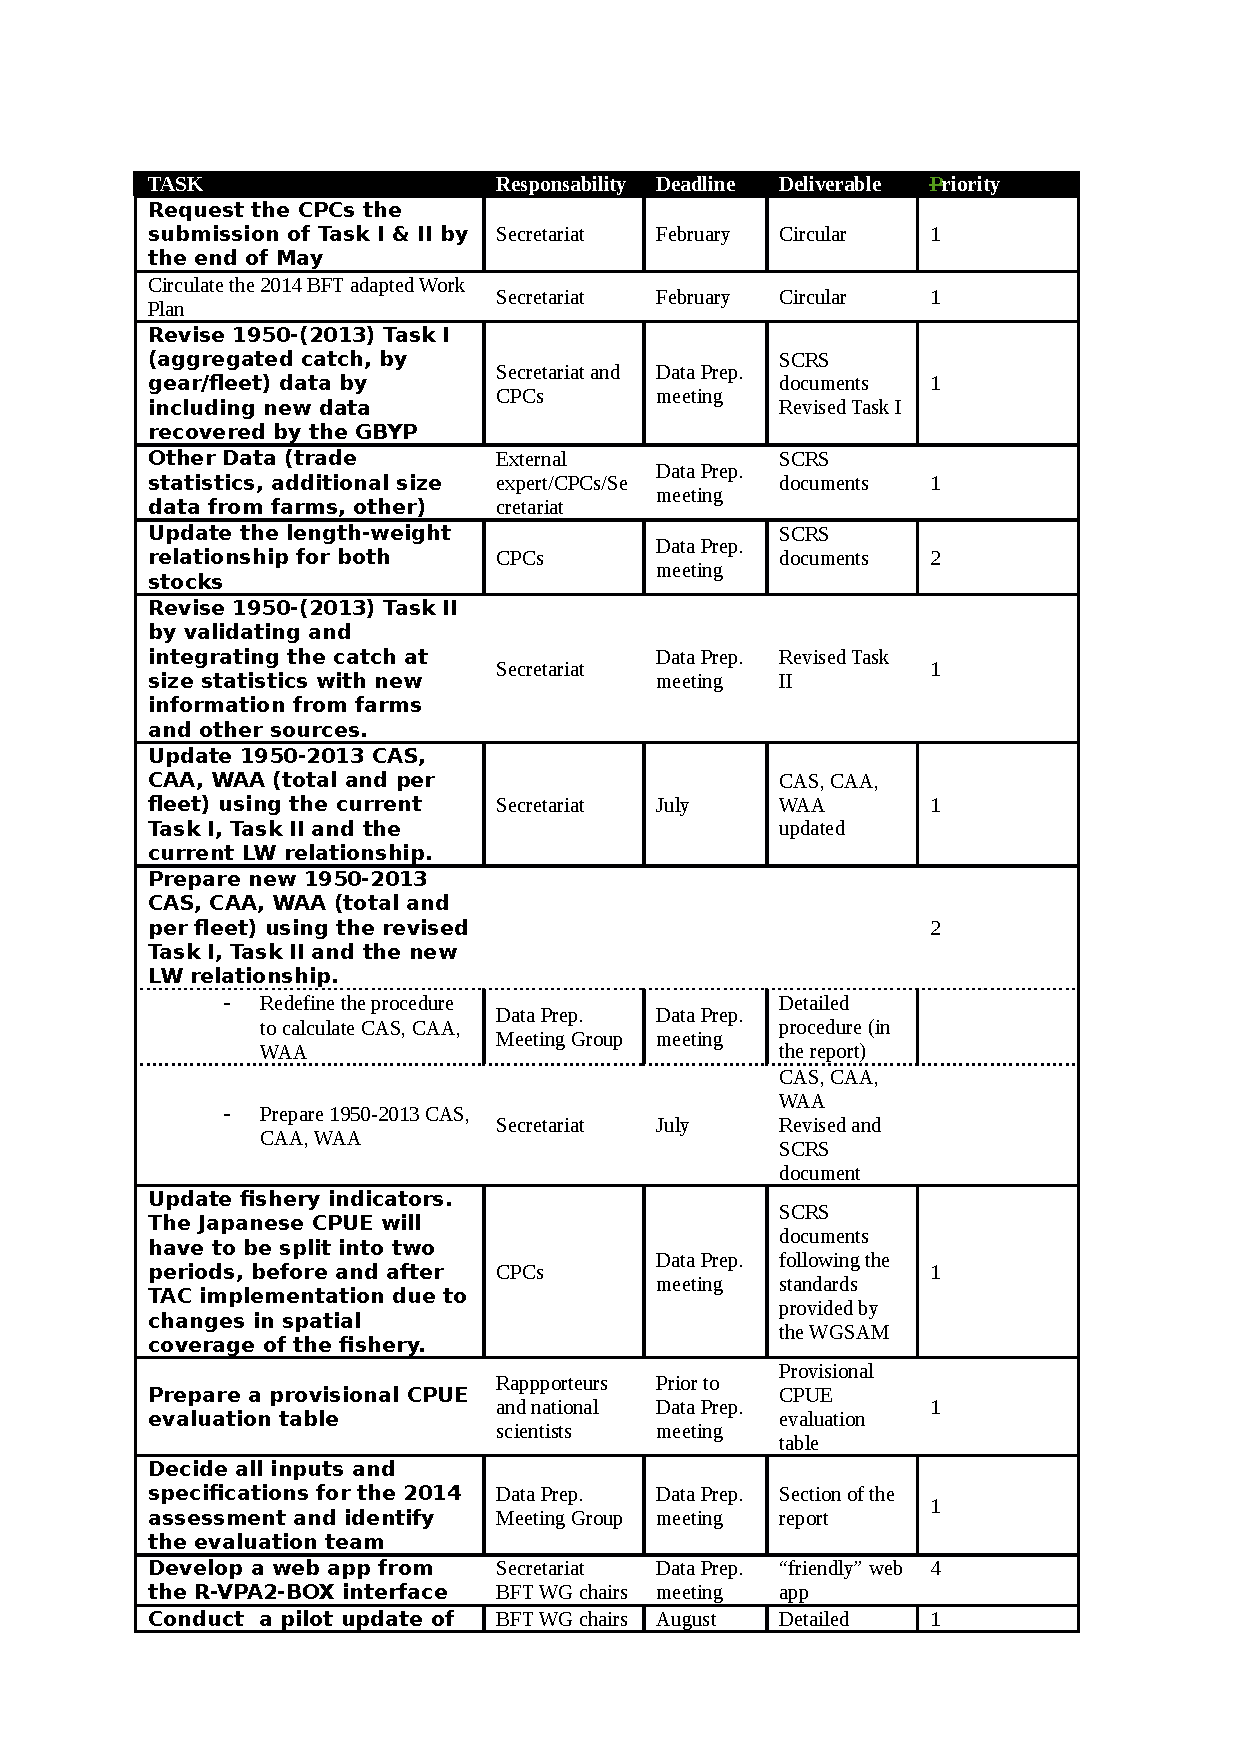
\includepdf[pages={1,2},lastpage=2]{dataPrepTab.pdf}
